\documentclass{beamer}

\usepackage{url}
\usepackage[english]{babel}
\usepackage{verbatim}
%%\usepackage{times}
%%\usepackage{graphicx}
\usepackage{lmodern}
\usepackage[utf8x]{inputenc}
\usepackage[T1]{fontenc}
\usepackage{listings}
\usepackage{mathtools}
\usepackage{color}
\usepackage{tikz}
\usetikzlibrary{arrows,shapes}

\mode<presentation>
{
  \definecolor{beamer@gker}{rgb}{0.8,0.0,0.0}
  \setbeamercolor*{structure}{fg=beamer@gker}
  \logo{\includegraphics[scale=0.5]{logo.pdf}}
}

\setbeamertemplate{footline}[text line]{%
  \parbox{\linewidth}{\vspace*{-8pt}
  \hfill
  %\insertshortauthor
  \hfill
  \insertframenumber\ of \inserttotalframenumber}}
\setbeamertemplate{navigation symbols}{}

\definecolor{light-gray}{gray}{0.60}

\title{Upcoming plans for pkg 1.4}
\author{Vsevolod Stakhov \\ \url{vsevolod@FreeBSD.org}}
\institute{\includegraphics[scale=0.5]{logo.pdf}}

\begin{document}

\begin{frame}[plain]
  \titlepage
\end{frame}

\begin{frame}
\frametitle{The list of main features}
\begin{itemize}
  \item Abstract repositories (ports, CPAN, CTAN\ldots)
  \item Flexible dependencies
  \item Package popularity contest
  \item Packaging of the base system
\end{itemize}
\end{frame}

\begin{frame}
\begin{center}
\huge{Abstract repositories}
\end{center}
\end{frame}

\begin{frame}
\frametitle{Repositories architecture}
\begin{figure}[h!]
  \centering
  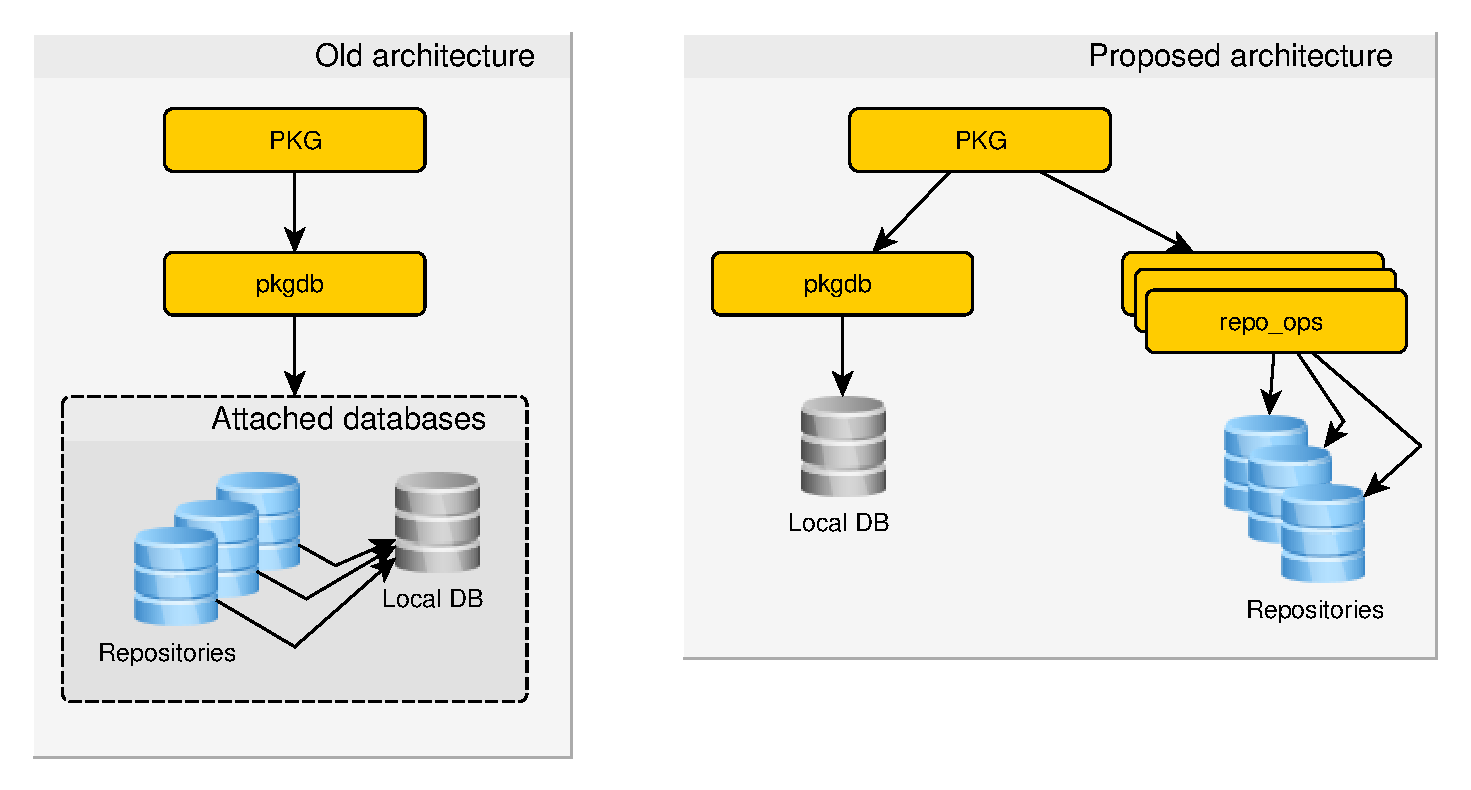
\includegraphics[width=0.99\textwidth]{flex_repos.pdf}
\end{figure}
\end{frame}

\begin{frame}
\frametitle{Abstract repositories}
Advantages of the new architecture.
\begin{itemize}
  \item No longer limited to sqlite3 repos.
  \item Better multirepo support (without attach hacks)
  \item Allows to create repostitories of many types:
  \begin{itemize}
    \item Ports
    \item C($T|R|P$)AN
    \item Base system?
    \item \ldots
  \end{itemize}
\end{itemize}
\end{frame}

\begin{frame}
\frametitle{Repository operations}
Repository operations.
\begin{table}[h]
\begin{tabular}{|l|p{6cm}|c|}
\hline
\textbf{Operation} & \textbf{Description} & \textbf{Mandatory} \\
\hline
\hline
Open & Opens repository & + \\
\hline
Init & Initialize repository structure & + \\
\hline
Create & Create repository & + \\
\hline
Close & Close repository & + \\
\hline
Update & Updates repository \footnote{this could be some cache building for some
repo types} & + \\
\hline
\end{tabular}
\end{table}
\end{frame}

\begin{frame}
\frametitle{Repository operations}
Packages operation
\begin{table}[h]
\begin{tabular}{|l|p{6cm}|c|}
\hline
\textbf{Operation} & \textbf{Description} & \textbf{Mandatory} \\
\hline
\hline
Query & Search for a package or packages & + \\
\hline
Shlib & Get information about provided or required shared libraries & - \\
\hline
Ensure\_loaded & Load specific fields of a package & + \\
\hline
Fetch & Fetch package from a repository\footnote{or compile it} & + \\
\hline
\end{tabular}
\end{table}
\end{frame}

\begin{frame}
\begin{center}
\huge{Flexible dependencies}
\end{center}
\end{frame}

\begin{frame}
\frametitle{New dependencies format}
\large{\[libblah >= 1.0 +option_1, +option_2 \| libfoo != 1.1\]}
\begin{itemize}
  \item Can depend on normal packages and virtual packages (provides)
  \item Easy to define the concrete dependency versions
  \item Alternative dependencies
\end{itemize}
\begin{figure}[h!]
  \centering
  \includegraphics[height=0.3\textheight]{q6.eps}
\end{figure}
\end{frame}

\begin{frame}
\frametitle{Flexible dependencies solving}
\begin{figure}[h!]
  \centering
  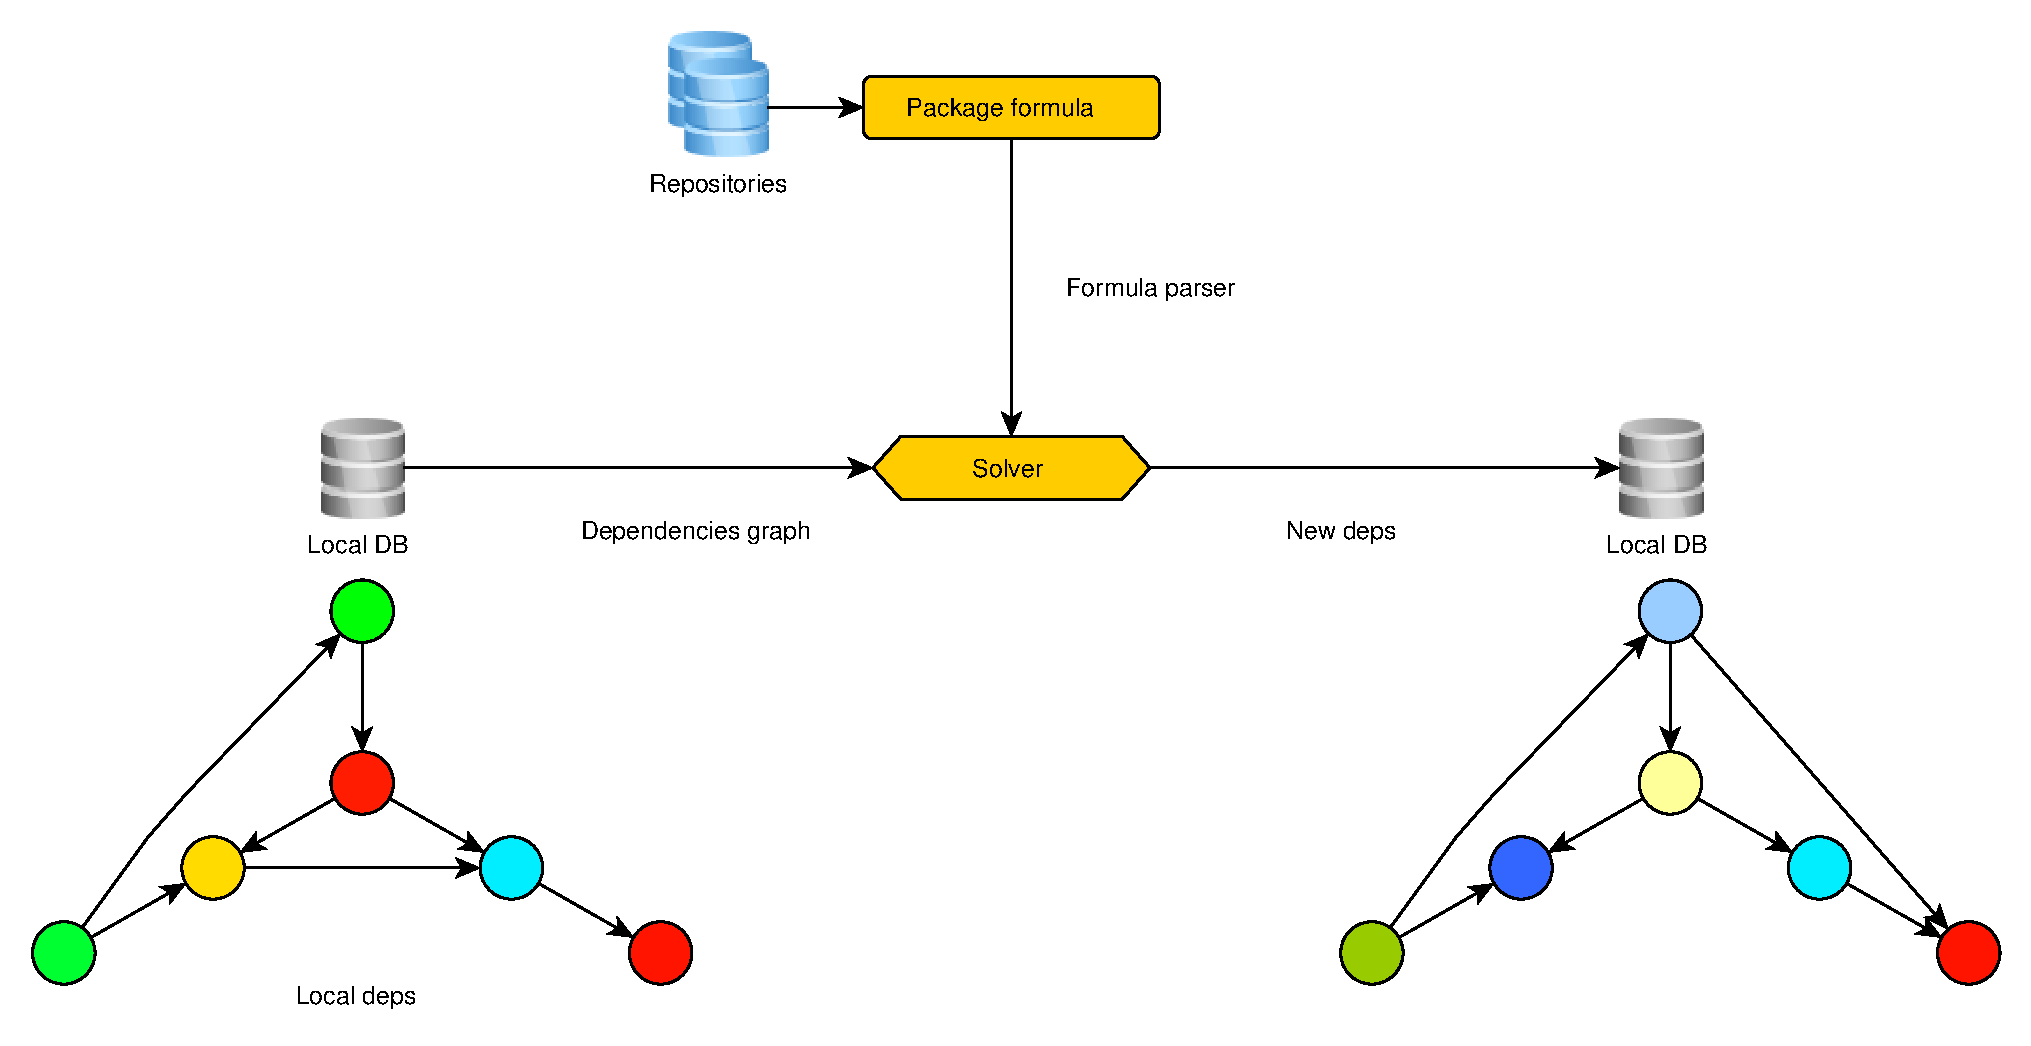
\includegraphics[width=0.99\textwidth]{flex_deps.pdf}
\end{figure}
\end{frame}

\begin{frame}
\begin{center}
\huge{Popularity contest}
\end{center}
\end{frame}

\begin{frame}
\frametitle{Purposes}
\begin{itemize}
  \item We want to gather statistics about packages using
  \item We can get statistics of OS versions/architectures
  \item We can check what options are mostly used
  \item We can estimate efficiency of security updates
\end{itemize}
\end{frame}

\begin{frame}
\frametitle{Problems with surveys}
\begin{enumerate}
  \item We must protect all statistical data transferred from active and passive
  attacks
  \item We must not ask for user's identity or establish it in any way
  \item We should be tolerate to keys compromising and provide forward secrecy
  \item We should protect server from malicious data and flooding
  \item We need to traverse throught NATs and corporate firewalls
\end{enumerate}
\end{frame}

\begin{frame}
\frametitle{Solution proposed}
\begin{itemize}
  \item Use EDH over HTTP requests as key exchange procedure
  \item Store long-term public key inside pkg binary (should be used for
  offline signing)
  \item Identify a client by some random UUID
  \item Suggest to a client some crypto puzzle:
  \begin{itemize}
    \item Relatively hard for unknown UUIDs
    \item Simpler puzzle for subsequent connections
    \item Very complex if submit rate from UUID is higher than normal 
  \end{itemize}
\end{itemize}
\end{frame}

\begin{frame}
\begin{center}
\huge{Packaging base}
\end{center}
\end{frame}

\begin{frame}
\frametitle{Problems arise}
\begin{enumerate}
  \item Too many build options available
  \item Number of packages from base system is not defined
  \item Need to export build options to system profile
  \item Configuration update and mergemaster need special care
\end{enumerate}
\end{frame}

\begin{frame}
\begin{center}
\includegraphics{logo.pdf} \\
\emph{Questions?} \\[4pt]
\url{vsevolod@FreeBSD.org}
\end{center}
\end{frame}
\end{document}